
\chapter{Background}
\label{chap:background}

This chapter explains the \textbf{basic concepts} used throughout the thesis. First, we explain \textbf{neural \acp{lm}}: from the basics of neural networks (§\ref{sec:nns}) and language modeling (§\ref{sec:lm-basics}), up to pretrained (§\ref{sec:plms}) and large language models (§\ref{sec:llms}). Then we move on to \textbf{\ac{d2t} generation}: covering rule-based (§\ref{sec:rule-d2t}) and neural-based systems (§\ref{sec:neural-d2t}), \ac{d2t} datasets (§\ref{sec:datasets}) and evaluation methods (§\ref{sec:evaluation}). We assume that the reader has certain expertise in related areas of \ac{nlp}, although not necessarily in \ac{nlg}. We aim to make the work self-contained by covering all the important concepts, pointing the interested reader to related work for more details.

Besides that, the chapter serves also as an \textbf{overview of the state of the art} in the fields of interest. In particular, the later subsections (\Cref{sec:plms,sec:llms} for neural \acp{lm} and \Cref{sec:neural-d2t,sec:datasets,sec:evaluation} for \ac{d2t} generation) describe the datasets, models, and metrics used for the experiments. As such, the chapter serves as the main point of reference; we will only briefly revisit the most relevant concepts in the respective chapters.


\section{Neural Language Models}
\label{sec:lms}
In this section, we work our way towards neural \acp{lm}: the mathematical foundations of \acp{nn} on which the neural \acp{lm} are built on (\autoref{sec:nns}), the basic ideas of language modeling (\autoref{sec:lm-basics}) and the way \acp{lm} are constructed, trained, and eventually applied in \ac{nlp} (\Cref{sec:plms,sec:llms}).

\subsection{Neural Networks}
\label{sec:nns}
First, we need to build a tool for learning patterns from data\footnote{Until we get to \ac{d2t} generation in \autoref{sec:d2t}, we will use the word ``\textit{data}'' only in its abstract sense, as in ``any inputs we can apply our algorithms to''. We will use the term ``structured data'' whenever it is necessary to make the distinction.}. This tool---which for us will be the \textbf{neural networks}---will later help us with learning patterns about language from large-scale textual data, and in turn with generating text.

Let's say our goal is to predict real-number output $y \in \mathbb{R}$ for the given vector of real numbers $\mathbf{x} = (x_1, \ldots, x_d) \in \mathbb{R}^d$.
% \footnote{We will follow the convention that vectors are denoted with boldface letters ($\mathbf{x}$), and real numbers with plain letters ($x$).} 
We assume that the $\mathbf{x} \rightarrow y$ mapping is not arbitrary (that would leave us with memorizing all the $(\mathbf{x},y)$ pairs), but follows some regularities and underlying patterns that can be learned. This assumption will be naturally satisfied if we consider $(\mathbf{x},y)$ to be representations of real-word data, e.g., documents and their labels.

For learning the underlying pattern between $\mathbf{x}$ and $y$, we will use mathematical models designed to capture the pattern in their parameters. The model estimates the parameters from a limited set of examples called the \textit{training data} and uses the learned parameters to predict the outputs on the \textit{test data}.

\paragraph{Perceptron Algorithm} One of the early mathematical models designed for predicting the outputs based on the inputs is the \emph{perceptron algorithm} (\citealp{rosenblatt1958perceptron}, \citealp[p.~192]{bishop2006pattern}). In this case, we assume the output is a binary class label: $y \in \{-1, 1\}$. The algorithm learns the parameters $\textbf{w} = (w_1, \ldots, w_d) \in \mathbb{R}^d$ and the bias $b \in \mathbb{R}$ describing a linear decision boundary separating the data points according to their class label. The algorithm proceeds as follows:


\begin{enumerate}
    \item The parameters $\textbf{w}$ and $b$ are initialized to small random values or zeros.
    \item For each training example $(\mathbf{x}_i, y_i)$, the algorithm updates the weights and bias to adjust their current estimate towards the ground truth target:
          \begin{align} \label{eq:perceptron1}
              \hat{y}_i  & = \text{sign}(\textbf{w} \cdot \mathbf{x} + b) \\
              \textbf{w} & = \textbf{w} + (y - \hat{y}) \textbf{x}        \\
              b          & = b + y - \hat{y}
          \end{align}
    \item The step (2) is repeated until convergence.
\end{enumerate}

The perceptron algorithm is guaranteed to converge if there exists a hyperplane which separates the data belonging to one class from another, otherwise it will not converge \cite{novikoff1962convergence}.

\paragraph{Multi-layer Perceptron} To overcome the fact that the perceptron is limited to linear decision boundaries, we can use a \textbf{\acl{mlp} (\acs{mlp}\glsunset{mlp}}; \citealp[p.~164]{goodfellow2016deep}). This mathematical model---also known as a feed-forward neural network---is able to approximate any bounded continuous function \cite{hornik1989multilayer}.

As the name suggests, \ac{mlp} uses multiple perceptron-like units called \textit{neurons}. Analogically to the perceptron (\autoref{eq:perceptron1}), each neuron computes its output $o$ using the rule:
\begin{align}
    o & = f(\mathbf{x}^\top \mathbf{w}  + b),
\end{align}
% \begin{itemize}
where $f: \mathbb{R} \rightarrow \mathbb{R}$ is the \emph{activation function}. Instead of signum, \ac{mlp} uses differentiable non-linear functions, most commonly nowadays \acl{relu} (\acs{relu}\glsunset{relu}; \citealp{nair2010rectified}) or its adapted version \acl{gelu} (\acs{gelu}\glsunset{gelu}; \citealp{hendrycks2016gaussian}).

For efficiency, the neurons are organized in layers, which enables formulating the \ac{mlp} computations in terms of matrix multiplication. The $i$-th layer of \ac{mlp} is parametrized with a matrix $\mathbf{W}_i \in \mathbb{R}^{d\times n}$ and a vector of biases $\mathbf{b}_i \in \mathbb{R}^{n}$, processing the \textit{hidden state} $\mathbf{h}_{i-1} \in \mathbb{R}^{d}$ (where we set $\textbf{h}_0 = \textbf{x}$):
\begin{align}
    \mathbf{h}_i & = f(\mathbf{h}_{i-1} \mathbf{W}_i + \mathbf{b}_i).
\end{align}
During training, we aim to minimize the \textit{loss function} describing the gap between the model predictions and the ground truth output. Since all the computations in \ac{mlp} are differentiable, we can use the chain rule to compute how each parameter in the network contributes to the loss. To minimize the loss, we use the \emph{backpropagation} algorithm \cite{kelley1960gradient,rumelhart1986learning}, updating the network parameters in the reverse order of layers. The magnitude of the updates is controlled by the learning rate parameter $\alpha$.

\paragraph{Recurrent Neural Networks} Unlike \acp{mlp}, where the size of the input is fixed, \acp{rnn} allow us to process a sequence of inputs $\mathbf{X} = (\mathbf{x}_1, \ldots, \mathbf{x}_n)$ of arbitrary length. Generally, an \ac{rnn} computes a sequence of hidden states $\mathbf{H} = (\mathbf{h}^{(0)}, \ldots, \mathbf{h}^{(n)})$ by repeatedly applying a function $f$ parametrized by the parameters of the network $\boldsymbol{\theta}$, the current input $\mathbf{x}_i$, and the previous hidden state $\mathbf{h}^{(i-1)}$ \cite[p.~367]{goodfellow2016deep}:
\begin{align}
    \mathbf{h}^{(i)} = f(\boldsymbol{\theta}, \mathbf{h}^{(i-1)}, \mathbf{x}_i).
\end{align}
The hidden state $\mathbf{h}^{(0)} \in \mathbb{R}^k$ is initialized randomly. After the input is processed, $\mathbf{H}$ contains an encoded representation of the sequence. The exact implementation of the function $f$ may vary, but is generally implemented as a series of matrix multiplications and non-linear functions.

Although \acp{rnn} are suitable for text processing and turned out to be have various successes in \ac{nlp} applications \TODO{cite}, they also have various shortcomings, including the limited dimensionality of the hidden state and limited possibilities of parallelization. However, they will serve as a stepping stone towards the transformer architecture described in \autoref{sec:lm-basics}.


\subsection{Text Representation}
\label{sec:lm-basics}
We will now look into the basics of text representation in neural networks.


\paragraph{One-Hot Encoding}
% Until now, we have assumed that the input to a network is a vector of real numbers. However, a
A text is a sequence of discrete units such as characters, words, or subwords. To convert these units---called \textit{tokens}---to a numerical representation, we can define a \textit{vocabulary} $V$ which assigns an integer index $i \in \{0, \ldots, |V|-1\}$ to each token.

The naive way to represent each token would be using its integer value. However, this would misleadingly suggest linear dependence between tokens. A better way is to use the index $i$ for constructing a \textit{one-hot} vector $\mathbf{x} \in \{0,1\}^{|V|} $ for each token:
\begin{align}
    x_j = \begin{cases}
        1 & \text{if } i = j, \\
        0 & \text{otherwise}.
    \end{cases}
\end{align}

While this representation is sound, it is quite sparse and does not capture the semantics of individual tokens, which puts high requirements on the representional capacity of the network.

\paragraph{Word Embeddings} To get a more useful representation of tokens, we may require that tokens with similar meaning are also close in the vector space. Using the distributional theory of meaning \cite{harris1954distributional,firth1957synopsis}, we can use the idea that tokens with similar roles also tend to occur in a similar context.

This idea is used in the Word2Vec algorithm \cite{mikolov2013distributed}. The algorithm extracts the token representations as the weights of an \ac{mlp} trained either for predicting the tokens in the neighborhood of each token (the \emph{skip-gram} objective) or vice versa, the token itself based on the tokens in its neighborhood (the \emph{continuous bag-of-words} objective). The output of the algorithm is an \textit{embedding matrix} $\mathbf{W}_e \in \mathbb{R}^{|V|\times d}$, which assigns each token a $d$-dimensional \textit{embedding vector} $\mathbf{x} \in \mathbb{R}^{d}$. The objectives are illustrated in \autoref{fig:word2vec}.

The idea of representing tokens with embedding vectors is employed in neural \acp{lm} described later in this section, even though the embedding matrix is not trained with the aforementioned algorithm, but joinly with the rest of the network.

\begin{figure*}[ht]
    \centering

    \begin{subfigure}{\textwidth}
        \centering
        \begin{subfigure}{0.45\textwidth}
            \centering
            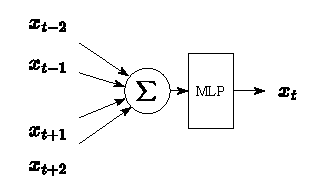
\includegraphics[width=\textwidth]{img/skipgram.pdf}
            \caption{Skip-gram}
            \label{fig:skipgram}
        \end{subfigure}
        \hspace{-20px}
        \begin{subfigure}{0.45\textwidth}
            \centering
            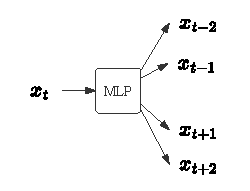
\includegraphics[width=0.75\textwidth]{img/cbow.pdf}
            \caption{Continuous Bag-of-Words}
            \label{fig:cbow}
        \end{subfigure}
    \end{subfigure}
    \caption{The objectives employed by the Word2Vec algorithm \cite{mikolov2013distributed}. In this case, the algorithm uses a context window of size $k=5$. In the (a) \emph{skip-gram} algorithm, we sum the embeddings of $k-1$ surrounding tokens and predict the original token. In the (b) \emph{continuous bag-of-words} algorithm, we use the original token for predicting the $k-1$ surrounding tokens.}
    \label{fig:word2vec}
\end{figure*}



\paragraph{Tokenization} We have also implicitly assumed that we have a way of splitting the text into tokens. Naively, we could split the text into words or characters. However, these approaches have their own shortcomings: word-level tokenization will not allow us to cluster together morphologically similar words, while character-level tokenization is computationally inefficient.

\emph{Subword tokenization}  is the middle ground between the two. The goal is to split the text into smaller pieces called \emph{subwords}, so that frequently used words will get their own subword, while less frequent words will be split into multiple subwords.

The subword tokenization algorithm that is frequently used in neural \acp{lm} is \emph{\ac{bpe}} \cite{sennrich2016neural}. The \ac{bpe} algorithm starts with the vocabulary of individual bytes, iteratively merging the most frequent tokens and adding them to the vocabulary $V$ until we reach the target vocabulary size. For example, the expression ``Subword tokenization'' could be split into four subwords \texttt{ ['Sub', 'word', '▁token', 'ization']}. The ``\texttt{▁}'' is a special character denoting a preceding space.


\subsection{Language Modeling}
Having a way to represent text, we can move on to processing it. Here, we will explain the notion of \emph{language modeling}.

\paragraph{Language Models} A useful formalism for text processing is a \emph{language model}: a mathematical model that estimates a probability of a sequence of tokens $X = (x_1, \ldots, x_n)$. For estimating the probability, we can factorize it into a product of conditional probabilities for each token using the chain rule:
\begin{align}
    P(X) = \prod_{i=1}^n P(x_i|x_1, \hdots, x_{i-1}).
\end{align}
Estimating the probability of longer sequences according to this formula is infeasible, as the model would require too many parameters. An \emph{\emph{n}-gram \ac{lm}} (parametrized by an integer \emph{N}) simplifies the product using the assumption that the probability of a token depends only on $N-1$ previous tokens:
\begin{align}
    P(X) = \prod_{i=1}^T P(x_i|x_{i-N+1}, \hdots,x_{i-1}).
\end{align}
The \emph{n}-gram \acp{lm} can be trained by estimating probabilities for individual \emph{n}-grams by tabulating their occurences in a text corpus. However, because of the limit on the length of the context for each token, the \emph{n}-gram \acp{lm} fail to capture long-term dependencies in the text.




\paragraph{Neural Language Model} A neural \ac{lm} is a \acl{lm} that estimates the text probability using a neural network. Denoting the parameters of the network by $\theta$, the probability of the sequence is given by the model probability distribution $P_\theta(X)$.

To learn $P_\theta(X)$, we minimize the cross-entropy between the model distribution $P_\theta$ and the empirical distribution of sequences in the corpus $P$:
\begin{align}
    H(P,P_\theta) = \mathbb{E}_P(-\log P_\theta) = -\sum_{\mathbf{x}\in C}p(X)\log p_{\theta}(X).
\end{align}

In contrast with \emph{n}-gram \acp{lm}, neural \acp{lm} can process the whole text, efficiently storing the probability estimates in its parameters, which makes it suitable for capturing long-term dependencies.

\subsection{Transformer Architecture}
\label{sec:transformer}
Here, we will pave our way towards the transformer architecture, which is a core neural architecture used for \ac{nlp} nowadays.

\paragraph{Encoder-Decoder Framework}
We have described an \ac{rnn} (\autoref{sec:nns}) as a neural network that can process the sequence and \emph{encode} its representation in a sequence of hidden states. The idea behind the \emph{encoder-decoder framework} \cite{sutskever2014sequence,cho2014learning} is that we can \emph{decode} an output sequence with another network using the last hidden state of the encoder as its initial state. With \acp{rnn}, the workflow is the following:

\begin{enumerate}
    \item The \textbf{encoder} encodes the sentence of input embeddings $\mathbf{X}= (\mathbf{x}_1, \ldots, \mathbf{x}_n)$ into a hidden state $\mathbf{h}_e$ by repeatedly applying a transformation $\mathcal{E}$ in each timestep $t\in(1,n)$:
          \begin{align}
              \mathbf{h}_e^{(i)} = \mathcal{E}(\mathbf{h}_e^{(i-1)}, \mathbf{x}_i).
          \end{align}
    \item The \textbf{decoder} uses $\mathbf{h}_e^{(n)}$ as its initial state $\mathbf{h}_d^{(0)}$ and produces the sequence of output tokens  $Y = (y_1, \ldots, y_m)$ by repeatedly applying a transformation $\mathcal{D}$ in each timestep $j\in(1,m)$:
          \begin{align}
              \mathbf{h}_d^{(j)}, y_j = \mathcal{D}(\mathbf{h}_d^{(j-1)}, y_{j-1}).
          \end{align}
\end{enumerate}

\paragraph{Attention Mechanism} We have already mentioned that the hidden state of an \ac{rnn} has a fixed size, which limits the amount of information the network can capture about a sequence. The \emph{attention mechanism} \cite{bahdanau2015neural} as used in \acp{rnn} enables the decoder to extract the information dynamically from the encoded sequence. In each step $j$, the decoder computes a context vector $c_j$ as the weighted sum of the hidden states of the encoder $\{\mathbf{h}_e^{(0)}, \ldots, \mathbf{h}_e^{(n)}\}$ using the attention matrix $\mathbf{W}_a$:
\begin{align}
    \alpha_{ji}  & = \operatorname{softmax}(\mathbf{h}_d^{(j)}\mathbf{W}_a \mathbf{h}_e^{(i)}), \\
    \mathbf{c}_j & = \sum_i \alpha_{ji} \mathbf{h}_e^{(i)}.
\end{align}
The context vector is used as an additional input for the decoder:
\begin{align}
    \mathbf{h}_d^{(j)}, y_j = \mathcal{D}(\mathbf{h}_d^{(j-1)}, y_{j-1}, \mathbf{c}_j).
\end{align}


\paragraph{Self-attention Mechanism} Self-attention \cite{cheng2016long,vaswani2017attention} is a variant of the attention mechanism in which the source and the target sequence is identical. For the input $\mathbf{X} \in \mathbb{R}^{n,d}$, the \emph{self-attention} produces the output $\mathbf{H} \in \mathbb{R}^{n,d}$ of the same size. For each token, the resulting vector $\mathbf{h}_i \in \mathbf{H}$ is a weighed combination of the value vectors corresponding to all the tokens in a sequence (including the token itself):
\begin{align}
    \mathbf{h}_j = \sum_{i\in 1..n} \alpha_{ji} \mathbf{v}_i,
\end{align}
where the \emph{value vector} of each token is computed using a trainable \emph{value matrix} $\mathbf{W_v} \in \mathbb{R}^{n,d}$:
\begin{align}
    \mathbf{v}_i = \mathbf{x}_i \mathbf{W_v}.
\end{align}
To get the attention weights $\alpha_{ij}$, we first compute \textit{query} and \textit{key} vectors for each token using trainable matrices $\mathbf{W_q}$ and $\mathbf{W_k} \in \mathbb{R}^{n,d}$. Each weight is then a normalized dot product of the corresponding vectors:
\begin{align}
    \mathbf{q}_i & = \mathbf{x}_i \mathbf{W_q}                                                      \\
    \mathbf{k}_i & = \mathbf{x}_i \mathbf{W_k}                                                      \\
    \alpha_{ij}  & = \operatorname{softmax}\biggl(\frac{\mathbf{q}_i\mathbf{k}_j}{\sqrt{d}}\biggr).
\end{align}
The operations can be efficiently paralellized using matrix multiplication:
\begin{align}
    \mathbf{Q}                                             = \mathbf{X}\mathbf{W_q},\quad\mathbf{K} & = \mathbf{X}\mathbf{W_k},\quad\mathbf{V} = \mathbf{X}\mathbf{W_v}                           \\
    \operatorname{Attn}(\mathbf{Q}, \mathbf{K}, \mathbf{V})                                         & = \operatorname{softmax}\biggl(\frac{\mathbf{Q}\mathbf{K}^\top}{\sqrt{d}}\biggr)\mathbf{V}.
\end{align}


\paragraph{Transformer Architecture} The \emph{transformer}\footnote{Although \citet{vaswani2017attention} uses ``Transformer'' with a capital ``T'', the orthography is gradually shifting towards the variant with a lower-case ``t''. See, e.g., \citet[p.~215]{jurafsky2024}.} \cite{vaswani2017attention} is a neural network architecture which can process sequences efficiently in parallel. To achieve that, the transformer replaces the \ac{rnn} hidden state (which previously served for sharing information among tokens in a single sequence) with the self-attention mechanism applied over a series of layers.

Specifically, each layer is composed of two sublayers: (a) the \emph{self-attention layer} and (b) the \emph{\ac{mlp} layer}. The output of the $i$-th sublayer is added to its original input $\mathbf{H}^{(i)}$ in a so-called residual connection:
\begin{align}
    \mathbf{H}^{(i+1)} = \mathbf{H}^{(i)} + \operatorname{sublayer}(\mathbf{H}^{(i)}).
\end{align}
The sublayers serve a different purpose: while the \ac{mlp} layer computes element-wise operations over each token, the self-attention layer enables sharing information among tokens. The sublayer input (or output, depending on the architecture variant) is normalized using \emph{layer normalization} \cite{ba2016layer}.

To get the input representation $\mathbf{H}^{(0)}$, we sum the token embeddings $\mathbf{X} \in \mathbb{R}^{n,d}$ with \emph{positional embeddings}. Positional embeddings encode the information about the absolute or relative position of individual tokens which would otherwise get lost in parallelized processing. See \citet{dufter2022position} for an overview of positional embedding variants.


\begin{figure*}[ht]
    \centering
    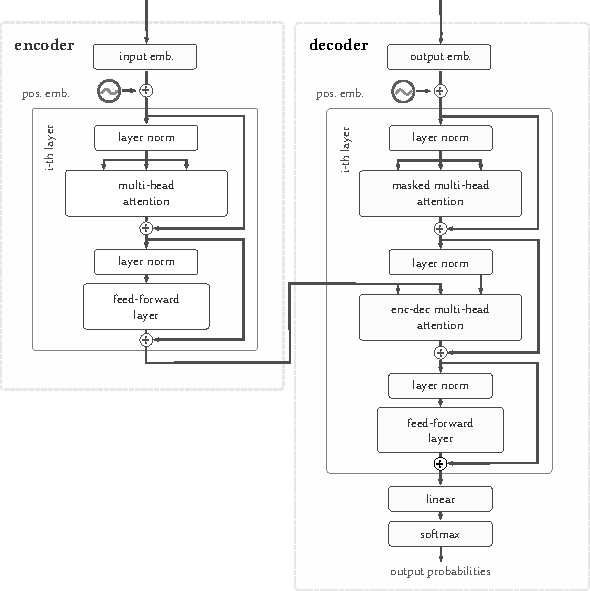
\includegraphics[width=0.9\textwidth]{img/transformer.pdf}
    \caption{An encoder-decoder variant of the Transformer architecture. The encoder has $N_{e}$ layers, each consisting of a self-attention and MLP sublayer. The decoder has $N_{d}$ layers with masked self-attention and encoder-decoder attention, again followed by an MLP sublayer. The input to each sublayer is normalized using layer norm. After the last decoder layer, the output probabilities are computed using a linear projection and softmax. The figure is adapted from \href{https://github.com/bbycroft/llm-viz/blob/main/src/llm/intro-image.svg}{https://github.com/bbycroft/llm-viz}.}
    \label{fig:transformer}
\end{figure*}


Training the transformer model is \emph{self-supervised}: each token in the training sequence serves as the ground-truth ``\emph{label}'' that the model aims to predict. For each token in the sequence, we train the model to maximize the log probability (i.e., minimize the negative log probability) of the ground truth token $x_i$ given the previous sequence of tokens in the sequence:
\begin{align}
    \operatorname{loss}_i = -\log P_\theta(x_i|x_1, \hdots, x_{i-1}).
\end{align}
We train the model on \emph{batches} of data, using an optimization algorithm such as \acl{sgd} (\acs{sgd}\glsunset{sgd}; \citealp[p.~275]{goodfellow2016deep}) or Adam \cite{kingma2014adam}. The batch size $b$ and the learning rate $\alpha$ are the training hyperparameters.

As shown in \autoref{fig:transformer}, the original Transformer architecture follows the encoder-decoder framework. The encoder layers follow an aforementioned scheme, while the decoder layers have the following differences:
\begin{itemize}
    \item Each layer contains another sublayer called the \emph{encoder-decoder attention}. In contrast to the self-attention mechanism, the \emph{keys} and \emph{values} come from the last layer of the encoder, enabling the decoder to attend to the encoded sequence.
    \item The self-attention is \emph{masked} so that each token can collect information only from the preceding tokens, which is necessary to enable text generation using left-to-right autoregressive decoding.
\end{itemize}
After the last decoder layer, the hidden states are projected into a matrix of size $\mathbb{R}^{|V|\times n}$ and normalized using softmax, producing a probability distribution over the vocabulary for each input token.

\paragraph{Text Generation} As we mentioned, we can use \textit{left-to-right autoregressive decoding} for generating text. The decoding process starts by feeding a special \texttt{<s>} (beginning of sequence) token into the decoder and then iteratively selecting the \emph{i}-th token based on the probability distribution for the \emph{i}-th position, until the  \texttt{</s>} (end of sequence) token is decoded. The procedure is outlined in Algorithm \ref{alg:decoding}.
\begin{algorithm}[ht]
    \begin{algorithmic}[1]
        \State{Initialize: $Y= \texttt{<s>}, y = \texttt{<s>}$ \Comment{Output sequence, current token}}
        \While{$y \neq \texttt{</s>}$}
        \State Predict next token probability distribution: $p(y | Y)$
        \State Sample next token: $t \sim p(y | Y)$ \label{alg:dec:sample}
        \State Update output sequence: $Y = Y \cup y$
        \EndWhile
        \State Return $Y$
    \end{algorithmic}
    \caption{Autoregressive decoding}
    \label{alg:decoding}
\end{algorithm}

\noindent The sampling step (line \ref{alg:dec:sample}) can be realized in various ways, including:
\begin{itemize}
    \item \textbf{Greedy decoding}: Select the most probable token: $y_i = \argmax{y \in V} p_\theta(y|\mathbf{y}_{<i}).$
    \item \textbf{Top-$k$ sampling}: Sample the next token from the $k$ most probable tokens.
    \item \textbf{Top-$p$ (nucleus) sampling} \cite{holtzman2019curious}: Sample the next token from the tokens with cumulative probability $p$.
    \item \textbf{Beam search}: Extend the $k$ most probable sequences from the previous step with the next tokens, keep the $k$ most probable sequences for the next step.
\end{itemize}
While the greedy decoding and beam search are used to decode more probable sentences, the sampling algorithms are used for decoding more creative outputs. The algorithms can be also combined together.

\subsection{Pretrained Language Models}
\label{sec:plms}
It turns out that training a transformer model from scratch is mostly not practical: it requires non-trivial computational resources, large-scale data sources, and extensive training time. The workflow that gradually established after the introduction of the transformer architecture is thus following: the models are first \emph{pretrained} using a generic objective on large-scale data, such as The Pile \cite{gao2020pile} or C4 \cite{raffelExploringLimitsTransfer2019}, and then \emph{finetuned} for downstream tasks on a task-specific dataset.

Although pretraining a model requires significant computational resources, \acp{plm} can be then made available for futher finetuning, which is more cost- and data- efficient.


\paragraph{Model types} Depending on the downstream task, different variants of the transformer architecture may be used for training a \ac{plm} (see \autoref{tab:pretrained_models} for an overview):

\begin{itemize}
    \item \textbf{Encoder models} -- The models use only the \emph{encoder} part of the transformer architecture. These models are trained using the \emph{\ac{mlm} objective}: predicting tokens on the masked positions in the sequence. The output of these models is a contextualized representation of the input sequence, which can be used for tasks such as sequence classification, sequence tagging, or computing sequence similarity.
    \item \textbf{Encoder-decoder models} -- The models use the original \emph{encoder-decoder} architecture. These models are usually trained using a variant of denoising objective: predicting the original sequence from its corrupted version. The models are mostly used for sequence-to-sequence tasks, such as \ac{mt}, question answering or summarization.
    \item \textbf{Decoder models} -- The models use only the \emph{decoder} part of the transformer architecture. These models are trained using the \emph{causal language modeling objective}: predicting the next token in a sequence. The models are suitable for unconditional text generation, but they can also used for the same tasks as the encoder-decoder models, using the input sequence as the ``pre-generated'' output prefix.
\end{itemize}

\begin{table}[t]
    \footnotesize
    \centering
    \begin{tabular}{lp{4.5cm}ll}
        \toprule
        \textbf{Type}            & \textbf{Pretraining Objective}            & \textbf{Model}                                       & \textbf{\# Parameters} \\
        \midrule
        \multirow{2}{*}{Encoder} & \multirow{2}{*}{Masked Language Modeling} & BERT \cite{devlinBERTPretrainingDeep2019}            & 110M-340M              \\
                                 &                                           & RoBERTa \cite{liuRoBERTaRobustlyOptimized2019}       & 125M-355M              \\
                                 &                                           & \textsc{LaserTagger} \cite{malmi2019lasertagger}     &                        \\
        \midrule
        \multirow{2}{*}{Enc-Dec} & \multirow{2}{*}{Text Denoising}           & BART \cite{lewisBARTDenoisingSequencetoSequence2019} & 139M-406M              \\
                                 &                                           & mBART \cite{liuMultilingualDenoisingPretraining2020} & 680M                   \\
                                 &                                           & T5 \cite{raffelExploringLimitsTransfer2019}          & 220M-11B               \\
        \midrule
        Decoder                  & Causal Language Modeling                  & GPT-2 \cite{radfordLanguageModelsAre2019}            & 117M-1.5B              \\
                                 &                                           & Llama2 \cite{touvronLlamaOpenFoundation2023}         & 7B-70B                 \\
                                 &                                           & Mistral \cite{jiangMistral7B2023}                    & 7B-70B                 \\
                                 &                                           & Zephyr \cite{tunstallZephyrDirectDistillation2023}   & 7B-70B                 \\
        \bottomrule
    \end{tabular}
    \caption{Types of transformer architectures, along with specific models used in this work. The number of parameters may vary based on the model variant.}
    \label{tab:pretrained_models}
\end{table}

\begin{figure*}[t]
    \centering
    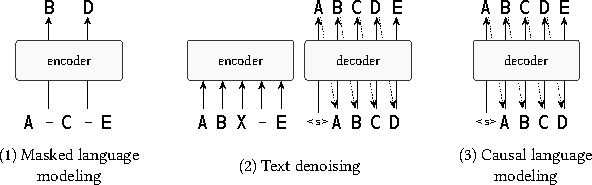
\includegraphics[width=0.9\textwidth]{img/objectives.pdf}

    \caption{A scheme of the common objectives used by pretrained models: 1) masked language modeling (encoder-only), 2) text denoising (encoder-decoder), 3)  causal language modeling (decoder-only). The special symbol \texttt{<s>} (beginning of a sentence) is used to bootstrap the decoding process.}\label{fig:objectives}

\end{figure*}

\paragraph{Finetuning} By \emph{finetuning} a model we mean additional training of a pretrained model on a task-specific dataset. Finetuning is more cost- and data-efficient than training a model from scratch, but is typically used only for a single task, since repeated model update can lead to erasing previous knowledge, also known as ``catastrophic forgetting'' \cite{mccloskey1989catastrophic,kirkpatrick2017overcoming}.


\paragraph{Few-shot and Zero-shot Settings} If the training data available to the model is very limited (no more than \textasciitilde 100 examples), we talk about a \emph{few-shot} setting. By taking it to the extreme, we arrive to a \emph{zero-shot} setting, in which we use a model on the task for which it has not been trained for. Making the models work in these settings is crucial for using the models in low-resource scenarios.

\subsection{Large Language Models}
\label{sec:llms}
Scaling the models in terms of the number of parameters and the size of the training data has turned out to further improve the performance of the models \cite{kaplan2020scaling,hoffmann2022training}. Larger models were shown to exhibit unprecedented capabilities in terms of language fluency, language understanding, and reasoning skills \cite{wei2022emergent,bubeck2023sparks}, giving name to a specific category of \emph{\aclp{llm} (\acsp{llm}\glsunset{llm};} \citealp{brown2020language,zhao2023survey}). \Acp{llm} are commonly larger than 1B parameters and based on the transformer decoder architecture. For many \ac{nlp} tasks, \acp{llm} have comparable or better performance than previous task-specific approaches.

\paragraph{In-context Learning} The general knowledge of \acp{llm} can be leveraged for performing on novel tasks without the need for finetuning on task-specific data. Instead, the task can be formulated in a natural language prefix (commonly called a \emph{prompt}), and the model completes the task by causal language modeling. This ability is known as \emph{in-context learning} \cite{brown2020language,dong2022survey}. If the model is given a limited set of input-output examples in the prompt, we talk about \emph{few-shot prompting}; if the model is given no examples, we talk about \emph{zero-shot prompting}.

\paragraph{Instruction Tuning} The key to strong cross-task of \acp{llm} is instruction tuning: finetuning on a large dataset of tasks formulated using natural language instructions, such as \textit{``Answer this question: \{question\}''} or \textit{``Translate this sentence: \{sentence\}''} \cite{sanh2021multitask,ouyang2022training}. The instruction-tuned models can be then easily \emph{prompted} to perform a task of choice in natural language, even if   they were not directly trained for the task.



\section{Data-to-Text Generation}
\label{sec:d2t}
In this section, we will provide background for the task of \ac{d2t} generation. After presenting the \ac{d2t} applications (\autoref{sec:d2t-tasks}) and the subtasks in the \ac{d2t} generation pipeline, we will discuss the rule-based (\autoref{sec:rule-d2t}), statistical (\autoref{sec:stat-d2t}), and neural (\autoref{sec:neural-d2t}) \ac{d2t} generation systems. Finally, we will describe the datasets (\autoref{sec:datasets}) and evaluation metrics (\autoref{sec:evaluation}) for \ac{d2t} generation used throughout this work.

\subsection{Applications}
\label{sec:d2t-tasks}

\ac{d2t} generation is a catch-all term for tasks which require \emph{mapping structured data to natural language}. The structured data can take various forms: tabular databases, graphs and knowledge bases, time-series, or charts \cite{gattSurveyStateArt2018,sharmaInnovationsNeuralDatatotext2022}. The \emph{form} of the input structured data is usually the defining feature of the \emph{dataset} (together with the related modeling approaches). Practical applications, on the other hand, may combine multiple data formats and approaches.

Here is a brief overview of applications of \ac{d2t} generation:

\begin{itemize}
    \item \textbf{Automated Journalism}: Augmenting (or in simple cases, even replacing) human journalists for writing data-based reports, including:
          \begin{itemize}
              \item \textbf{News reports}: Automating news writing, e.g., for election results \cite{leppanen2017data}, incidents \cite{vanderleeCACAPODatasetMultilingual2020}, earthquakes \cite{oremus2014first}, or wildlife tracking \cite{siddharthan2012blogging,ponnamperuma2013tag2blog}.
              \item \textbf{Sport reports}: Generating game summaries for sports such as basketball \cite{wiseman2017challenges,thomson2020sportsett}, baseball \cite{puduppullyDatatotextGenerationEntity2019}, or soccer \cite{van2017pass}.
              \item \textbf{Financial reports}: Supporting financial decisions by generating comments on stock prices \cite{murakami2017learning,aoki2018generating} or summaries of financial documents \cite{chapman2022towards}.
              \item \textbf{Weather reports}: Generating weather forecasts and weather-related reports \cite{goldberg1994using,belz2005corpus,belz2008automatic,angeli-etal-2010-simple,balakrishnan2019constrained}.
          \end{itemize}
    \item \textbf{Business Intelligence Reports}: Providing decision support in business reports alongside data summaries and visualizations (mostly commercial companies such as \href{https://www.arria.com}{Arria}, \href{https://infosentience.com}{InfoSentience}, or \href{https://www.vphrase.com}{vPhrase}; also \citealp{perlitzDiversityEnhancedTabletoText2022}; see \citealp{daleNavigatingTextGeneration2023} for a recent overview),
    \item \textbf{Chart Captioning}: Generating captions\footnote{In contrast to image captioning \cite{stefanini2022show}, here the systems can rely on the underlying data in textual form (although the approaches can be hybrid, see e.g. \citealp{kantharajCharttoTextLargeScaleBenchmark2022}).} for charts or graphs, e.g., for assistive technologies, document indexing, or simplifying decision support \cite{demirGeneratingTextualSummaries2008,demirSummarizingInformationGraphics2012,obeidCharttoTextGeneratingNatural2020,kantharajCharttoTextLargeScaleBenchmark2022}.
    \item \textbf{Healthcare Summaries}: Providing  clinical data summaries about patients to clinicians \cite{portet2009automatic,scott2013data}, or vice versa, providing medical information to patients, e.g., for behavioral change \cite{reiter2003lessons} or nutritional counseling \cite{balloccu-reiter-2022-comparing}.
    \item \textbf{Product Descriptions}: Automating generating product descriptions in specific domains such as for laptops and TVs \cite{wen2015toward,wen2016multi}, or general-domain approaches for big e-commerce platforms \cite{shaoControllableDiverseText2021,kotoCanPretrainedLanguage2022}.
\end{itemize}

\subsection{D2T Generation Pipeline}
\label{sec:d2t-pipeline}


Until recently, \ac{d2t} generation could not be realized in end-to-end fashion. Typically, the systems decomposed the task into of approximately 4-6 subtasks\footnote{Some tasks may be further subdivided, which can generate up to 10 subtasks as in \citet{milleModD2TMultilayerDataset2023}.} \cite{reiterBuildingAppliedNatural1997,reiterArchitectureDatatoTextSystems2007,gattSurveyStateArt2018}. Here we selected five representative subtasks illustrated in \autoref{fig:pipeline}:

\begin{enumerate}
    \item \textbf{Content Selection}: Deciding which facts from the structured data
          to include in the text.
    \item \textbf{Document Planning}: Determining the order of the
          facts, dividing the facts into paragraphs.
    \item \textbf{Sentence Planning}: Aggregating the facts into
          sentences.
    \item \textbf{Lexicalisation}: Transforming the facts to text segments.
    \item \textbf{Surface Realisation}: Combining the text segments into a well-formed text in natural language.
\end{enumerate}


\begin{figure*}[t]
    \centering
    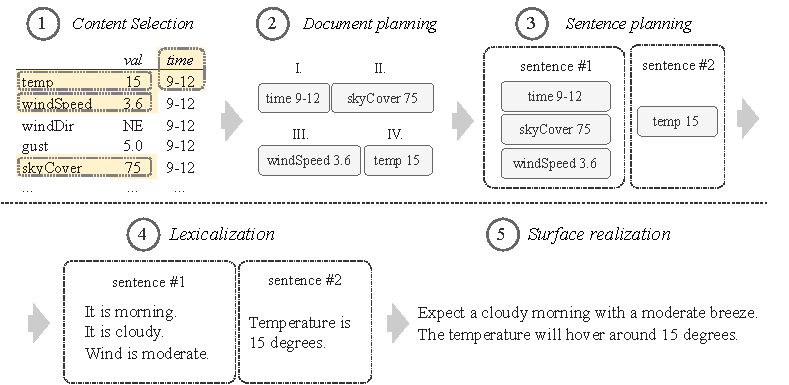
\includegraphics[width=\textwidth]{img/pipeline.pdf}

    \caption{TODO}\label{fig:pipeline}

\end{figure*}


Decomposing \ac{d2t} generation into subproblems---where each module tackles a simple task---helps to modularize the system. Since each module has a specific and well-defined function, it makes the system as a whole more explainable. Modularization also enables realizing each part of the system using a different approach (see \Cref{sec:rule-d2t,sec:stat-d2t,sec:neural-d2t}).

The subtasks are typically executed in a \emph{pipeline}, meaning the input is sequentially processed by individual modules. The pipeline-based approach can lead to error accumulation, propagating errors to downstream modules. Despite these issues, the pipeline approach remain widely used in practice
%  a cornerstone approach for grammar-based surface realization systems such as  and it is employed in software frameworks such as SimpleNLG \cite{gatt2009simplenlg}. 
and also brings benefits to neural-based systems \cite{ferreiraNeuralDatatotextGeneration2019}, as we will explore in \autoref{sec:pipeline}.


\subsection{Rule-based Approaches}
\label{sec:rule-d2t}

By \emph{rule-based approaches} for \ac{d2t} generation, we mean approaches which require manual construction of rules or grammars for tackling the task, as opposed to data-driven approaches. It is useful to view these approaches through the lens of the \ac{d2t} generation pipeline (\autoref{sec:d2t-pipeline}) as a way to built module for individual subtasks. Rule-based approaches, especially in combination with other approaches, are still in use in various forms today \cite{gattSurveyStateArt2018,daleNaturalLanguageGeneration2020,daleNavigatingTextGeneration2023}.


\paragraph{Content Selection and Text Planning} The rules for the earlier stages of the \ac{d2t} generation pipeline are typically domain-specific, relying on the judment of domain experts. In the content selection step, heuristics can be used for extracting important information from the data, e.g., \textit{``if a pattern is detected in the signal, include it in the report''} \cite{portet2009automatic}. Various factors can influence the decision, including target length of the goal summary, the problem at hand, or the target audience \cite{gkatziaContentSelectionDatatoText2016}. In the text planing step, discourse strategies are designed for satisfying the desired communicative goals such as \emph{define}, \emph{compare}, or \emph{describe}, which emerge from domain-specific schemata \cite{mckeown1985text}. The resulting rules are typically in the form \textit{``if a player scores two consecutive goals, describe these in the same sentence''}  \cite{gattSurveyStateArt2018}.


\paragraph{Template-based Lexicalization} Simpler rule-based approaches for lexicalization and surface realization are characterised by \emph{templates}: pre-written text snippets which are ``glued'' together and filled with values from the data. Templates can range from simple fill-in-the-blank approaches (such as \textit{``The temperature will be \{temp\} degrees''}) to more sophisticated templates using a templating language \cite{reiter2016nlg,gatt2009simplenlg}.  Hand-written rules are used not only for selecting the templates, but also combining them and filling the placeholders with values (where the latter can be non-trivial in languages with rich morphology). The resulting rule-based system is usually tied to the specific task and domain and cannot handle more complex cases, but can be way to generate sufficient outputs with reasonable development time and costs \cite{vanderleeAutomatedLearningTemplates2018}.


\paragraph{Grammar-based Lexicalization} For handling more complex cases, we can use grammar-based approaches. Even though a \emph{grammar} is technically also a set of rules, it describes the production rules for the whole sentence without relying on templates.
% \footnote{Even though a \emph{grammar} is technically also a set of rules, here we mention it separately since it is a generic approach which can describe the production rules for the whole sentence without relying on templates.} 
Grammar-based approaches are rooted in linguistic theories such as systemic grammars \cite{halliday1985systemic,matthiessen1991lexico} or meaning-text theory \cite{mel1988dependency,goldberg1994using,milleModD2TMultilayerDataset2023}, and typically rely on off-the-shelf realizers such as FUF/SURGE \cite{elhadad1997surge} or KPML \cite{bateman1997enabling}. Grammar-based approaches are more general-purpose than rule-based approaches, but require considerable amount of manual effort into building the systems, tend to require very detailed
input, and often need additional rules for choosing among related options \cite{gattSurveyStateArt2018}.
% FORGe \cite{milleFORGeWebNLG20172017,mille2019teaching}


\subsection{Statistical Approaches}
\label{sec:stat-d2t}

Statistical \ac{d2t} generation overlaps with classical machine learning methods, and these approaches are therefore better described as \emph{pre-neural data-driven} approaches. The idea of statistical approaches is to \emph{estimate the parameters} for a particular task using statistics of a text corpus.

This idea is not mutually exclusive with rule-based and grammar-based approaches. In fact, the first statistical approaches used statistics for re-ranking the lexical realization outputs generated from a grammar-based system \cite{bangalore2000corpus,langkilde2000forest,ratnaparkhi2000trainable}, or even integrated the statistical information directly at the level of generation decisions \cite{belz2008automatic}. Fully data-driven approaches then still relied on grammatical rules, only the rules were derived from treebanks: for example the approach of \citet{white2007towards} relied on a Combinatory Categorial Grammar \cite{steedman2001syntactic} derived from the Penn Treebank \cite{hockenmaier2007ccgbank}. Oftentimes, the particular approach was hybrid, combining a set of hand-written rules or grammars together with statistical models \cite{konstas2012concept,gardent2017statistical}.

For the earlier stages of the \ac{d2t} generation pipeline, various unsupervised machine learning methods were used. \citet{duboue2003statistical} proposed to use a clustering-based method for content selection, estimating the relative important of each cluster for the final text. \citet{barzilay2004catching} then modelled the content structure using Hidden Markov Models \cite{baum1966statistical}, learning the structure from unannotated documents. Learning latent variables can be used for learning alignment between the text and the data, which in turn helps with text segmentation and structuring \cite{liang2009learning}.

\subsection{Neural Approaches}
\label{sec:neural-d2t}
Naturally extending the work on statistical \ac{d2t} generation, neural networks (see \autoref{sec:nns}) began replacing other data-driven approaches around 2015. With their renewed capabilities, mostly due to advances in hardware \cite{hooker2021hardware} and capabilities of learning from large data \cite{lecun2015deep}, they enabled not only building more powerful modules for the \ac{d2t} generation pipeline, but also replacing the pipeline entirely with end-to-end models.

The field of neural \ac{d2t} generation is broad, as it has been gaining a lot of interest in the recent years, with works covering many deep learning-related concepts \cite{sharmaInnovationsNeuralDatatotext2022, lin2023survey}. Here, we will mainly focus on concepts and model architectures related to this thesis, and we will further describe works related to individual datasets in \autoref{sec:datasets}.


\paragraph{Linearization} For getting an input sequence suitable for the neural model, the structured data needs to be linearized as a sequence of tokens. To preserve the original structure of data, a common practice is to use special tokens serving as delimiters, as depicted in \TODO{figure}. Linearization can be very effective \cite{yang2020improving,hoyle2021promoting,xieUnifiedSKGUnifyingMultiTasking2022}, beating specialized encodings designed to process the particular structure \cite{marcheggianiDeepGraphConvolutional2018,koncel-kedziorskiTextGenerationKnowledge2019}.

An alternative to linearization is to use special embeddings for the structural elements (e.g., for table rows and columns), which are summed with the positional and token embeddings \cite{wang2021tuta,yangTableFormerRobustTransformer2022}. Since the embeddings need to be learned, the approach is more suitable for high-resource tasks.

\paragraph{Delexicalization} In many cases, a particular data value may appear only few or zero times in the training data. The data scarcity makes it difficult for the model to learn how to work with the value. Delexicalization is the process of replacing entities with placeholders, essentially working with the fill-in-the-blank templates \cite{oh2000stochastic,mairesse2010phrase,wen2015semantically,dusekSequencetoSequenceGenerationSpoken2016}.  The blanks are filled later in the post-processing step. This approach was shown useful even for languages with rich morphology, where the values can be filled using a separate language model \cite{duvsek2019neural}.

\paragraph{Sequence-to-Sequence Generation} Generating text from data in the end-to-end fashion, i.e., without intermediate steps, is enabled by neural \ac{seq2seq} models. \Ac{seq2seq} models are designed for transforming variable-length input sequences into variable-length output sequences \cite{cho2014learning,sutskever2014sequence}. The typical \ac{seq2seq} architecture is the encoder-decoder framework described in \autoref{sec:transformer}. In the case of \ac{d2t} generation, the input sequence is the linearized version of structured data and the output sequence is the target text.

\paragraph{RNN-based Approaches} The original seq2seq approaches designed for \ac{mt} \cite{cho2014learning,sutskever2014sequence} were soon adopted for other \ac{nlg} tasks. Using structured representation of the dialogue act as the input, \citet{wen2015semantically} use \acp{rnn} to generate the response in a dialogue system. On a similar task, \citet{dusekSequencetoSequenceGenerationSpoken2016} show that it is better to generate output strings with a \ac{rnn}-based system directly instead of combining the model with a separate surface realization system. For generating weather reports, \citet{mei2016talk} use \acp{rnn} to also address the content selection step, identifying salient data records using the attention mechanism.

An important addition to the \ac{rnn}-based approaches was the \emph{copy mechanism} \cite{gu2016incorporating,seeGetPointSummarization2017}. The mechanism allows the model to copy tokens directly from the input. As used by \citet{gehrmannEndtoEndContentPlan2018}, it serves as an alternative to delexicalization, delegating the job of filling the entities to the model and making the process learnable.

\acp{rnn} were still used even after the introduction of the transformer model (\autoref{sec:transformer}), since they tended to work better in the low-resource settings. \citet{freitagUnsupervisedNaturalLanguage2018} experimented with using text denoising as an objective pretraining an \ac{rnn}-based system for \ac{d2t} generation. For adapting an \ac{rnn}-based model to other domains, \citet{wen2020recurrent} proposed \emph{data counterfeiting}, i.e., replacing delexicalized slots with slots from another domain. To reduce hallucinations, \citet{rebuffel2021controlling} the decoder considers content, hallucination and fluency scores via 3 RNNs, hidden states are summed

Various shared tasks and comparisons \cite{gardentWebNLGChallengeGenerating2017,dusekEvaluatingStateoftheartEndtoEnd2020,ferreiraNeuralDatatotextGeneration2019} showed that RNN-based approaches were generally competitive with rule-based approaches. The RNNs produce more fluent text, while the pipeline-based approaches made less semantic errors.


\paragraph{PLM-based Approaches} Using a transformer model for \ac{d2t} generation became practical with the arrival of \acp{plm} (see \autoref{sec:plms}). For example, the 2020 WebNLG+ shared task \cite{ferreira20202020}, with the goal of generating text from graph-structured triples (see \autoref{sec:datasets}), was dominated by systems based on pretrained encoder-decoder transformer models (\citealp{yang2020improving,agarwalMachineTranslationAided2020,kasnerTrainHardFinetune2020}; see \autoref{sec:plms}).

The general knowledge of language, along with the learned ability to copy tokens from the input, made it possible to get rid of both \emph{delexicalization} and \emph{copy mechanism}, while having the model handle rare entities not present in the task-specific training data. Transformer-based pretrained models are also able to produce outputs with considerably better fluency than \ac{rnn}-based models. On top of that, the variants of \acp{plm} pretrained on multilingual corpora are able to handle outputs in a variety of languages \cite{liuMultilingualDenoisingPretraining2020,xueMT5MassivelyMultilingual2021}.

Due to the aforementioned advantages, \ac{plm}-based approaches excel in low-resource settings, which is a default setup for many \ac{d2t} generation tasks. Following \citet{chenFewShotNLGPreTrained2019}, other works adopted PLMs for few-shot or zero-shot D2T generation. The models are generally finetuned on the domain-specific data for few-shot generation \cite{changNeuralDatatoTextGeneration2021,suFewShotTabletoTextGeneration2021}, or on the related domains for zero-shot generation \cite{kasner2022neural,kasnerMindLabelsDescribing2022}.

Improving \ac{plm}-based \ac{d2t} generation revolves around (1) finding suitable \emph{data representations}, and (2) ensuring the \emph{semantic accuracy} of the outputs. The data representations are closely related to the particular datasets, which we discuss in \autoref{sec:datasets}, while the semantic accuracy is related to the evaluation metrics, which we discuss in \autoref{sec:evaluation}. \ac{plm}-based \ac{d2t} generation is also discussed in detail in the recent surveys of \citet{sharmaInnovationsNeuralDatatotext2022} and \citet{lin2023survey}, to which we refer for more details.

\paragraph{LLM-based Approaches} At the time of writing, using \acp{llm} for \ac{d2t} generation is still in its naissance. The works that compared zero-shot or few-shot \ac{llm} prompting with finetuned \acp{plm} on existing datasets have found that the \acp{llm} rank behind state-of-the-art finetuned models on automatic metrics \cite{axelssonUsingLargeLanguage2023,yuanEvaluatingGenerativeModels2023}. We have shown that \acp{llm} can be employed for zero-shot generation of data in standard data formats, the main issue still being semantical accuracy of the outputs \cite{kasnerReferenceBasedMetricsAnalyzing2024}. However, there are yet no large-scale comparisons or attempts of finetuning \acp{llm} for \ac{d2t} generation.

% There are multiple factors which complicate benchmarking \acp{llm} on \ac{d2t} generation. Using closed \acp{llm}, which are accessible only through an API \cite{openai2023gpt4,chatgpt}, makes the work non-reproducible. Evaluation is also complicated with potential data contamination: the fact that any existing benchmark (including its test set) may have been included in the pretraining data of \acp{llm} \cite{golchin2023time,aiyappa-etal-2023-trust,balloccu2024leak}.

% On the other hand, \acp{llm} hold the promise of further simplifying data processing, enabling .

\subsection{Datasets}
\label{sec:datasets}

In this section, we outline the format and structure of \ac{d2t} generation datasets, focusing on the datasets used later on in the thesis. See \autoref{tab:datasets} for an overview. We do not describe our novel datasets presented in \citet{kasnerMindLabelsDescribing2022} and \citet{kasnerReferenceBasedMetricsAnalyzing2024}; these are described in their respective sections in \autoref{chap:investigating}.

\begin{table*}[t]
    \centering\small
    \begin{tabular}{@{}lllr@{}}
        \toprule
        \textbf{Dataset}                                                                           & \textbf{Data Format} & \textbf{Domain(s)}      & \textbf{\# Ex.} \\  \midrule
        CACAPO \cite{vanderleeCACAPODatasetMultilingual2020}                                       & Key-value            & News$^\blacklozenge$    & 20,149          \\
        DART \cite{nan2021dart}                                                                    & \ac{rdf} triples     & Wikipedia$^\lozenge$    & 70,524          \\
        \textbf{E2E} \cite{dusekSemanticNoiseMatters2019,dusekEvaluatingStateoftheartEndtoEnd2020} & Key-value            & Restaurants             & 36,856          \\
        EventNarrative \cite{colas2021eventnarrative}                                              & \ac{rdf} triples     & Events$^\lozenge$       & 224,428         \\
        HiTab \cite{chengHiTabHierarchicalTable2021}                                               & Table w/hl           & Statistics$^\lozenge$   & 10,672          \\
        Chart-To-Text \cite{kantharajCharttoTextLargeScaleBenchmark2022}                           & Table                & Statistics$^\lozenge$   & 34,811          \\
        Logic2Text \cite{chenLogic2TextHighFidelityNatural2020}                                    & Table w/hl           & Wikipedia$^\lozenge$    & 10,753          \\
        LogicNLG \cite{chenLogicalNaturalLanguage2020}                                             & Table                & Wikipedia$^\lozenge$    & 37,015          \\
        NumericNLG \cite{suadaaTabletoTextGenerationNumerical2021}                                 & Table                & Science$^\lozenge$      & 1,355           \\
        SciGen \cite{moosaviLearningReasonText2021}                                                & Table                & Science$^\lozenge$      & 17,551          \\
        \textbf{Rotowire} \cite{wiseman2017challenges}                                             & Table                & Basketball              & 6,150           \\
        ToTTo \cite{parikhToTToControlledTableToText2020}                                          & Table w/hl           & Wikipedia$^\lozenge$    & 136,553         \\
        \textbf{WebNLG} \cite{gardentWebNLGChallengeGenerating2017}                                & \ac{rdf} triples     & DBPedia$^\blacklozenge$ & 42,873          \\
        WikiBio \cite{lebretNeuralTextGeneration2016}                                              & Key-value            & Biographies$^\lozenge$  & 728,321         \\
        WikiSQL \cite{zhong2017seq2sql}                                                            & Table + SQL          & Wikipedia$^\lozenge$    & 80,654          \\
        WikiTableText \cite{bao2018table}                                                          & Key-value            & Wikipedia$^\lozenge$    & 13,318          \\
        \bottomrule
    \end{tabular}
    \caption{The list of \ac{d2t} datasets used in this work. The datasets are included in the \textsc{TabGenie} framework (\autoref{sec:tabgenie}), the datasets in \textbf{boldface} are also used in other experiments. Glossary of data types: \textit{Key-value}: key-value pairs, \textit{Graph}: subject-predicate-object triples, \textit{Table}: tabular data (\textit{w/hl}: with highlighted cells), \textit{Chart}: chart data, \textit{SQL}: strings with SQL queries. $\blacklozenge$ indicates that the dataset is multi-domain; $\lozenge$ indicates that the dataset is open-domain.}
    \label{tab:datasets}.
\end{table*}

\paragraph{Data Formats} Structured data come in several common formats with minor variations. The most common formats are:

\begin{itemize}
    \item \textbf{Key-value pairs}: Each input is a set of tuples $(k, v)$, where $k$ is a key (also called a slot), which is typically a text string, and $v$ is a value, which can be a text string, and number, or a combination of these. It is often used as \emph{\ac{mr}} (e.g., for dialogue states or dialogue acts) in dialogue systems.
    \item \textbf{\acs{rdf} (\Acl{rdf})\footnote{See \url{https://www.w3.org/TR/PR-rdf-syntax/}.} triples}: Each input is a set of triples $(s, p, o)$, where $s$ is a \emph{subject},  $p$ is a \emph{predicate}, and $o$ is an \textit{object}. A subject is usually an entity (person, object, or place), an object is either also an entity, or a generic text string or a number. A predicate expresses the relation between the subject and the object. This formalism can be also used to describe a \emph{directed graph} (e.g., a knowledge graph), where $s$ and $o$ are nodes and $p$ is a directed edge between these nodes.
    \item \textbf{Table}: Each input is structured as a \textit{table}, i.e., a two-dimensional cell matrix of $m$ columns and $n$ rows. Cells can be divided between headings (containing a ``key'' for the respective row or column), or contain a textual or numerical value. A subset of cells may be \emph{highlighted } -- in that case, the output text should describe only that particular subset of cells. A generalized version of a table may also contain merged cells, nested headings, or multiple disjoint table regions.
\end{itemize}

As we show in \autoref{chap:tabgenie}, all of the aforementioned formats can be unified in a tabular format with minimal information loss. In \autoref{sec:prompting}, we also show how to handle data in the JSON format.\footnote{JavaScript Object Notation; see \url{https://www.json.org}.} Other data formats, which we do not consider here, include \ac{amr}

\paragraph{Domains} The notion of a \emph{domain} is usually understood in \ac{d2t} generation under the \href{https://dictionary.cambridge.org/dictionary/english/domain}{Cambridge Dictionary} definition ``an area of interest''. However, the term may be slippery: while \citet{wen2016multi} consider the domains so related as \emph{TVs} and \emph{laptops} as distinct, \citet{lin2023survey} considers the tables from ACL Anthology papers \cite{suadaaTabletoTextGenerationNumerical2021} as domain-specific.

Most commonly, the term \emph{multi-domain} is used if the content of two subsets of data comes from a different distributions, so that a model train on one subset does not straighforwardly generalize to another (see, e.g., \citealp{vanderleeCACAPODatasetMultilingual2020,budzianowskiMultiWOZLargeScaleMultiDomain2020,rastogiScalableMultiDomainConversational2020}). If the topic of the dataset is unrestricted, or if it is based on a large-scale data source such as Wikipedia, the datasets is then considered \emph{open-domain} (see, e.g., \citealp{chenLogicalNaturalLanguage2020,nan2021dart,kann2022open}).

\paragraph{Datasets} The following datasets are the most relevant for the thesis:

\begin{itemize}
    \item \textbf{WebNLG}: The WebNLG dataset \cite{gardentCreatingTrainingCorpora2017,gardentWebNLGChallengeGenerating2017} contains \ac{rdf} triples from DBPedia \cite{auer2007dbpedia} and their crowdsourced descriptions. Each example consists of 1-7 triples, together forming a subgraph in the DBPedia knowledge graph. The target text should describe all the entities and the relations between them. The original WebNLG dataset \cite{gardentCreatingTrainingCorpora2017} contains 15 domains, out of which 5 are \emph{unseen}, i.e., included only in the test set (Athlete, Artist, MeanOfTransportation, CelestialBody, Politician). Each set of triples included several verbalizations to promote lexical variability. The dataset has been iteratively fixed, annotated for intermediate subtasks, and enriched with semi-automated German translations \cite{castroferreiraEnrichingWebNLGCorpus2018}. The version 3.0 \cite{ferreira20202020} contains one additional domain and automatic translations to Russian.
          \begin{itemize}
              \item
                    The dataset has been used in a series of shared tasks called \emph{WebNLG Challenge} \cite{gardentWebNLGChallengeGenerating2017,shimorinaWebNLGChallengeHuman2019,ferreira20202020,cripwell2023WebNLGShared2023}, out of which we participated in the 2020 edition (\citealp{ferreira20202020}; see \autoref{sec:finetuning}). We also used the dataset in the experiments on low-resource \ac{d2t} generation (\Cref{sec:iterative,sec:pipeline}), evaluation (\autoref{sec:sem-acc}), data processing (\autoref{sec:tabgenie}), and out-of-domain generalization (\autoref{sec:describing}).
          \end{itemize}

    \item \textbf{E2E}: The E2E dataset \cite{dusekEvaluatingStateoftheartEndtoEnd2020} contains restaurant descriptions in the form of key-value pairs (3-8 items per example) and corresponding human-written restaurant recommendations. The name of the dataset is derived from the E2E Challenge, a shared task that focused on evaluating end-to-end \ac{d2t} generation systems. Since original version of the dataset contained semantic noise (incorrect or missing facts in the crowdsourced descriptions), we use the cleaned version from \citet{dusekSemanticNoiseMatters2019} as the default version for our experiments.
          \begin{itemize}
              \item
                    Similarly to WebNLG, we used the dataset in the experiments on low-resource \ac{d2t} generation (\Cref{sec:iterative,sec:pipeline}), evaluation (\autoref{sec:sem-acc}), and data processing (\autoref{sec:tabgenie}).
          \end{itemize}

    \item \textbf{Rotowire}: Rotowire \cite{wiseman2017challenges} is a dataset with tabular statistics of basketball games and their corresponding game summaries. The target text contains only a subset of the input data (not highlighted a priori), so the systems need to model \emph{content selection} as well. Together with the above-average length of the target summaries, this aspect makes the dataset particularly challenging for \ac{d2t} generation systems.
          \begin{itemize}
              \item
                    We used the outputs from the neural systems on this dataset for building a token-level evaluation metric (\autoref{sec:eval-token}), and we included its updated version SportSett:Basketball \cite{thomson2020sportsett} in our data processing toolkit (\autoref{sec:tabgenie}).
          \end{itemize}
\end{itemize}



\subsection{Evaluation Metrics}
\label{sec:evaluation}

The most common evaluation measures for \ac{d2t} generation are \emph{intrinsic}, i.e., focusing on evaluating certain aspects of the quality of the system and its outputs \cite{gkatzia2015snapshot,celikyilmazEvaluationTextGeneration2021}.\footnote{As opposed to \emph{extrinsic} measures, which evaluate the impact of the system in the external environment \cite{celikyilmazEvaluationTextGeneration2021}. While \emph{extrinsic} metrics could give us better picture of the real-world impact, they are not suitable for early research stages due to high demands on the system quality, and they are also less suitable for evaluating individual subtasks \cite{van2019best}.} On a high-level, the intrinsic measures can be grouped between \emph{automatic metrics} and \emph{human evaluation}. Automatic metrics are generally cheaper, faster, and more replicable, but often serve only as a crude heuristic for the desired performance measure. Human evaluation is more expensive and difficult to execute, but if executed correctly, it can give us a more precise and fine-grained picture of system performance. A rule of thumb is that an experimental result should be supported by both kinds of metrics.


If we have human-written (also called \emph{ground truth} or \emph{golden}\footnote{\emph{Golden} refers to the fact that the systems usually try to imitate human performance. However, see \citet{clarkAllThatHuman2021} or \citet{dusekSemanticNoiseMatters2019} for examples where human-written references are not the desired correct reference, especially when gathered by crowdsourcing platforms.}) reference texts at our disposal, we can use \emph{reference-based}  automatic metrics. Here, the implicit assumption is that more similar the generated text is to the respective human-written reference text, the better. \emph{Referenceless} metrics, on the other hand, can be more varied: they can either judge the intrinsic qualities of the text such as text fluency, text diversity, and reading level, or---taking the input data into account---the faithfulness of the text with respect to the input data.


\paragraph{Lexical Similarity} Lexical similarity metrics measure the similarity between the generated and reference text using their word-level overlap. The metrics are fast, easy to compute, and have been used for decades as a convenient proxy for system comparison in various \ac{nlp} areas \cite{celikyilmazEvaluationTextGeneration2021}. However, there is a recent upsurge of works arguing against these metrics, because their correlations with human judgements for high quality outputs are low or negative, and the metrics fail to capture fine-grained phenomena \cite{mathurTangledBLEUReevaluating2020,kocmiShipNotShip2021,gehrmannRepairingCrackedFoundation2022}. As a general rule, lexical similarity metrics (which are still useful, e.g., for comparison with prior work) should be accompanied by other metrics.

Here are some of the common metrics which we use in this work:

\begin{itemize}
    \item \textbf{BLEU} \cite{papineni2002bleu} measures $n$-gram precision, i.e., to which extent do the $n$-grams in the generated text correspond to the reference text.  It is computed as a geometric mean of the $n$-gram precisions, with a brevity penalty to penalize shorter outputs. BLEU has been originally used for evaluating \ac{mt}, but since then it has become commonplace in \ac{nlp}. The SacreBLEU library \cite{post2018call}  was developed to tackle inconsistencies in implementations of the metric.
    \item \textbf{ROUGE} \cite{lin-2004-rouge} is a set of metrics which focus on recall, i.e., to which extent does the generated text preserve the information in the reference text. ROUGE has been originally designed for evaluating automatic summarization, but similarly to BLEU, it has been used widely (and as recently found by \citet{gruskyRogueScores2023}, oftentimes incorrectly) across the \ac{nlp} literature. ROUGE includes several variants, such as ROUGE-L, which measures the longest matching word sequence, and ROUGE-{1/2/3/4}, which measures the overlap on the respective n-grams.
    \item \textbf{METEOR} \cite{banerjee-lavie-2005-meteor} is a metric which computes harmonic mean of precision and recall computed on unigrams. METEOR also partially addresses semantic similarities of texts by using stemming and synonym matching. It has been shown to produce better correlations with human judgements than BLEU \cite{agarwal2008meteor}, but is more complex and expensive to compute.
    \item \textbf{NIST} \cite{martin2000nist} is a metric which focuses on precision similarly to BLEU. Howeveer, ot assigns lower weights to less common n-grams, which are considered less informative \cite{doddington2002automatic}, and its length penalty is more robust to small variations in text length.
    \item \textbf{ChrF++} \cite{popovic2015chrf,popovic2017chrf} is a metric which computes the F1-score on character $n$-grams. The metric is more robust to morphological variations than word-level metrics. On top of the original ChrF metric, Chrf++ also takes word unigrams and bigrams into account.
          % \item \textbf{CIDEr} \cite{vedantam2015cider} is a metric originally designed for evaluating image captions. It considers n-gram overlap, word frequency, and the informativeness of the generated caption compared to the reference captions. While not typically used for text summarization or \ac{mt} evaluation, it can be adapted for these tasks as well.
\end{itemize}
\paragraph{Semantic Similarity} Semantic similarity metrics measure the semantic similarity of the generated and reference texts, particularly using their distributional semantics \TODO{cite}. Going beyond lexical resemblance has only become possible with word embeddings (see \autoref{sec:lm-basics}), especially their contextual variant computed by pretrained \ac{rnn} or transformer encoders (\citealp{peters2018deep,devlinBERTPretrainingDeep2019}; see \autoref{sec:transformer}). The metrics are more robust with respect to the lexical variations, but are more computationally expensive and subject to the limitations of pretrained models' biases and black-box nature.

Here are the metrics which we consider in this work:

\begin{itemize}
    \item \textbf{BERTScore} \cite{zhang2019bertscore} measures semantic similarity of the texts by computing cosine similarity between the embeddings of the texts encoded by a pretrained transformer model. It was originally developed on top of BERT \cite{devlinBERTPretrainingDeep2019}, but it now supports other transformer encoder models. Its flexibility helps to achieve better correlations with human judgment, but makes it less suitable for intra-work comparison.
    \item \textbf{BLEURT} \cite{sellam2020bleurt} measures semantic similarity using a BERT model \cite{devlinBERTPretrainingDeep2019} which is further finetuned on synthetically labeled data. The similarity is again computed as a cosine similarity of the contextual embeddings. Compared to BERTScore, BLEURT is less flexible but ensures more consistent setup across works.
    \item \textbf{NUBIA} \cite{kaneNUBIANeUralBased2020} measures semantic equivalence of texts by combining features from two finetuned RoBERTa models \cite{liuRoBERTaRobustlyOptimized2019}---on the semantic similarity benchmark STS \cite{cer-etal-2017-semeval} and on the natural language inference benchmark MNLI \cite{williams2018mnli}---and the perplexity from the GPT-2 model \cite{radford2019language}. These features are combined with an \ac{mlp} layer. Combining the features ensures even better robustness of the metric at the cost of higher complexity and higher computational requirements.
\end{itemize}

\paragraph{Semantic Accuracy} Semantic accuracy---also called \emph{faithfulness} or \emph{factual consistency} \cite{celikyilmazEvaluationTextGeneration2021}---measures inacurracies in the output text with respect to the input data. The inacurracies can be broadly divided into \emph{omissions} (the model not mentioning facts in the input data) and hallucinations (the model mentioning extra facts that are not supported by the input data). Naturally, omissions apply only if the task requires to mention all the facts present in the input data. Further, the hallucinations can be \emph{extrinsic}, i.e., the model introduces external information not present in the data, or \emph{intrinsic}, i.e., the model uses the data incorrectly \cite{maynezFaithfulnessFactualityAbstractive2020}.

There are no widely accepted metrics for measuring semantic accuracy in \ac{d2t} generation. The closest notion is the \emph{slot error rate} from task-oriented dialogue systems, which is typically implemented by exact string match or regular expressions  \cite{wen2015semantically,dusekEvaluatingStateoftheartEndtoEnd2020}. For tabular data, the PARENT \cite{dhingraHandlingDivergentReference2019} was proposed as a reference-based metric, which uses lexical alignment models for computing precision and recall for tabular values.  In \Cref{sec:sem-acc,sec:eval-token}, we present two novel \emph{referenceless} metrics for evaluating semantic accuracy of \ac{d2t} generation using \acp{plm}. In \autoref{sec:prompting}, we also show how to evaluate semantic accuracy of texts using a prompted \ac{llm}.

\paragraph{Text Fluency} Text fluency is a catch-all term for measuring grammatical correctness, spelling, word and stylistical choices of text \cite{celikyilmazEvaluationTextGeneration2021}. Since texts more similar to the human written text tend to be more fluent, lexical and semantic similarity metrics (such as BLEU) are often used as a proxy for measuring text fluency. Alternatively, we can use the \emph{perplexity} of the text under a neural \ac{lm}, assuming that the \ac{lm} assigns lower probability to less probable sentences \cite{leeFactualityEnhancedLanguage2022,kaneNUBIANeUralBased2020}.


\paragraph{Lexical Diversity} Lexical diversity measures the variability and richness of expressions in the text \cite{vanmiltenburgMeasuringDiversityAutomatic2018}. One way to express the lexical diversity is the ratio between the average number of different words and the total number of words, called \emph{\ac{ttr}} or simply \emph{distinct $n$-grams} \cite{johnson1944studies,li2016diversity}. We can also measuring conditional entropy of the $n$-grams \cite{shannon1948mathematical}.
Lexical diversity is not generally required for \ac{d2t} generation, although there are approaches explicitly aiming to decode diverse outputs \cite{hanGeneratingDiverseDescriptions2021,perlitzDiversityEnhancedTabletoText2022}.

\paragraph{Human Evaluation} Since automatic metrics serve only as imperfect proxies for human judgment, using \emph{human annotators} is a crucial part of any \ac{nlg} experimental evaluation \cite{gehrmannRepairingCrackedFoundation2022}. Although are attempts at standardizing human evaluation \cite{thomsonGoldStandardMethodology2020}, human annotation protocols are usually task-specific \cite{van2019best,belzDisentanglingPropertiesHuman2020}. There are two main paradigms of human evaluation: large-scale evaluation using crowd workers focusing mostly on quantitative aspects (\emph{crowdsourcing}), and small-scale evaluation using expert annotators focusing mostly on qualitative aspects (\emph{manual evaluation}).

\begin{itemize}
    \item \textbf{Crowdsourcing}: Crowdsourcing platforms such as Amazon Mechanical Turk\footnote{\url{https://www.mturk.com}} or Prolific\footnote{\url{https://prolific.com}} are often used for distributing the work between human annotators. These platforms offer a convenient interface for hiring annotators with a specific background and ensuring that the annotators are paid fair wage. Due to financial incentives, the quality of outputs may vary, especiallysince the workers may nowadays be tempted to use \acp{llm} for certain tasks \cite{veselovskyArtificialArtificialArtificial2023}. It is therefore necessary to employ quality assurance checks in the annotation process.
    \item \textbf{Manual Evaluation}: To measure fine-grained aspects of output quality, manual evaluation---done either by the paper authors or other domain experts---may be employed. The goal of manual evaluation is to provide insights into the kind of errors that appear in the output texts, using a small or moderate-size sample of data (20-100 examples).
\end{itemize}


\paragraph{LLM-based Evaluation} Recently, researchers have started to examine the potential of replacing human workers with \acp{llm} \cite{zhaoInvestigatingTabletoTextGeneration2023,sottanaEvaluationMetricsEra2023,kocmiLargeLanguageModels2023,chiang-lee-2023-large,wangChatGPTGoodNLG2023a,fu2023gptscore}. In particular, the GPT-4 model \cite{openai2023gpt4} was shown to be capable of following fine-grained instructions compared to other LLMs and to have high correlations with human judgment on evaluating generated texts. Using \acp{llm} can be cheaper and more robust compared to using human annotators, especially since the model can be prompted for the specific task. However, there concerns about its non-reproducibility \cite{kocmiGEMBAMQMDetectingTranslation2023} and potential bias of these models \cite{wangLargeLanguageModels2023}.